
\section{Principal Components Analysis in R}

There are two functions in R for carrying out PCA -
\lstinline!princomp()! and \lstinline!prcomp()!. The
\lstinline!princomp()! function uses the \lstinline!eigen()! function to
carry out the analysis on the covariance matrix or correlation matrix,
while \lstinline!prcomp()! carries out an equivalent analysis, starting
from a data matrix, using a technique called singular value
decomposition (SVD). The SVD routine has greater numerical accuracy so
it should generally be preferred but we'll delay it's use until next
week when we introduce the mathematics behind SVD. The
\lstinline!princomp()! function is also useful when you don't have
access to the original data, but you do have a covariance or correlation
matrix (a frequent situation when re-analyzing data from the
literature). By default the \lstinline!princomp()! function carries out
PCA on the covariance matrix of the data. If you wish to carry out PCA
using the correlation matrix specify the argument \lstinline!cor=T!.

To demonstrate PCA we'll use Anderson's Iris data set.

\begin{R}
> names(iris)
[1] "Sepal.Length" "Sepal.Width"  "Petal.Length" "Petal.Width"  "Species"     
> iris
    Sepal.Length Sepal.Width Petal.Length Petal.Width    Species
1            5.1         3.5          1.4         0.2     setosa
2            4.9         3.0          1.4         0.2     setosa
3            4.7         3.2          1.3         0.2     setosa    
.. output truncated ..
> summary(iris) # notice that  Petal.Width is
        # about an order of magnitude smaller than the other variables.
        # We should therefore consider doing the PCA on the correlation
        # matrix rather than the cov matrix. We'll try both
> setosa <- subset(iris, Species=='setosa', select=-Species)        
> pca.setosa <- princomp(setosa)
> summary(pca.setosa)
Importance of components:
                          Comp.1    Comp.2    Comp.3     Comp.4
Standard deviation     0.4813799 0.1902114 0.1620508 0.09408823
Proportion of Variance 0.7647237 0.1193992 0.0866625 0.02921456
Cumulative Proportion  0.7647237 0.8841229 0.9707854 1.00000000
> plot(pca.setosa) # plots histogram plot of eigenvalues
> plot(pca.setosa$scores)  # in space of PC1 and PC2
> plot(pca.setosa$scores, asp=1)  # compare to the previous plot     
> plot(pca.setosa$scores[,1],pca.setosa$scores[,3], asp=1) # PC1 and PC3
> pca.setosa$loadings

Loadings:
             Comp.1 Comp.2 Comp.3 Comp.4
Sepal.Length -0.669 -0.598  0.440       
Sepal.Width  -0.734  0.621 -0.275       
Petal.Length        -0.490 -0.832 -0.240
Petal.Width         -0.131 -0.195  0.970

               Comp.1 Comp.2 Comp.3 Comp.4
SS loadings      1.00   1.00   1.00   1.00
Proportion Var   0.25   0.25   0.25   0.25
Cumulative Var   0.25   0.50   0.75   1.00

# now do the PCA based on the correlation matrix
> pca.setosa.cor <- princomp(setosa,cor=T)
> summary(pca.setosa.cor)
Importance of components:
                          Comp.1    Comp.2    Comp.3     Comp.4
Standard deviation     1.4347614 1.0110283 0.8172027 0.50145917
Proportion of Variance 0.5146351 0.2555446 0.1669551 0.06286532
Cumulative Proportion  0.5146351 0.7701796 0.9371347 1.00000000
> pca.setosa.cor$loadings

Loadings:
             Comp.1 Comp.2 Comp.3 Comp.4
Sepal.Length  0.604  0.335         0.720
Sepal.Width   0.576  0.441        -0.689
Petal.Length  0.375 -0.627 -0.677       
Petal.Width   0.403 -0.548  0.733       

               Comp.1 Comp.2 Comp.3 Comp.4
SS loadings      1.00   1.00   1.00   1.00
Proportion Var   0.25   0.25   0.25   0.25
Cumulative Var   0.25   0.50   0.75   1.00
> plot(pca.setosa.cor)
> plot(pca.setosa.cor$scores,asp=1)
\end{R}

\begin{assignment}
Do a PCA analysis on the iris data set with all
three species pooled together. Generate a plot showing the projection of
the specimens on the first two PC axes as shown in the figure below.
Represent the specimens from a given species with different colors. Make
sure you include a legend for your plot.

\medskip
Apply PCA (on the covariances) to the \lstinline!yeast-subnetwork! data
set from week three. Now do the same analysis based on PCA of the
correlation matrix. How does your interpretation of the data change?
\end{assignment}


\begin{figure}[htbp]
\centering
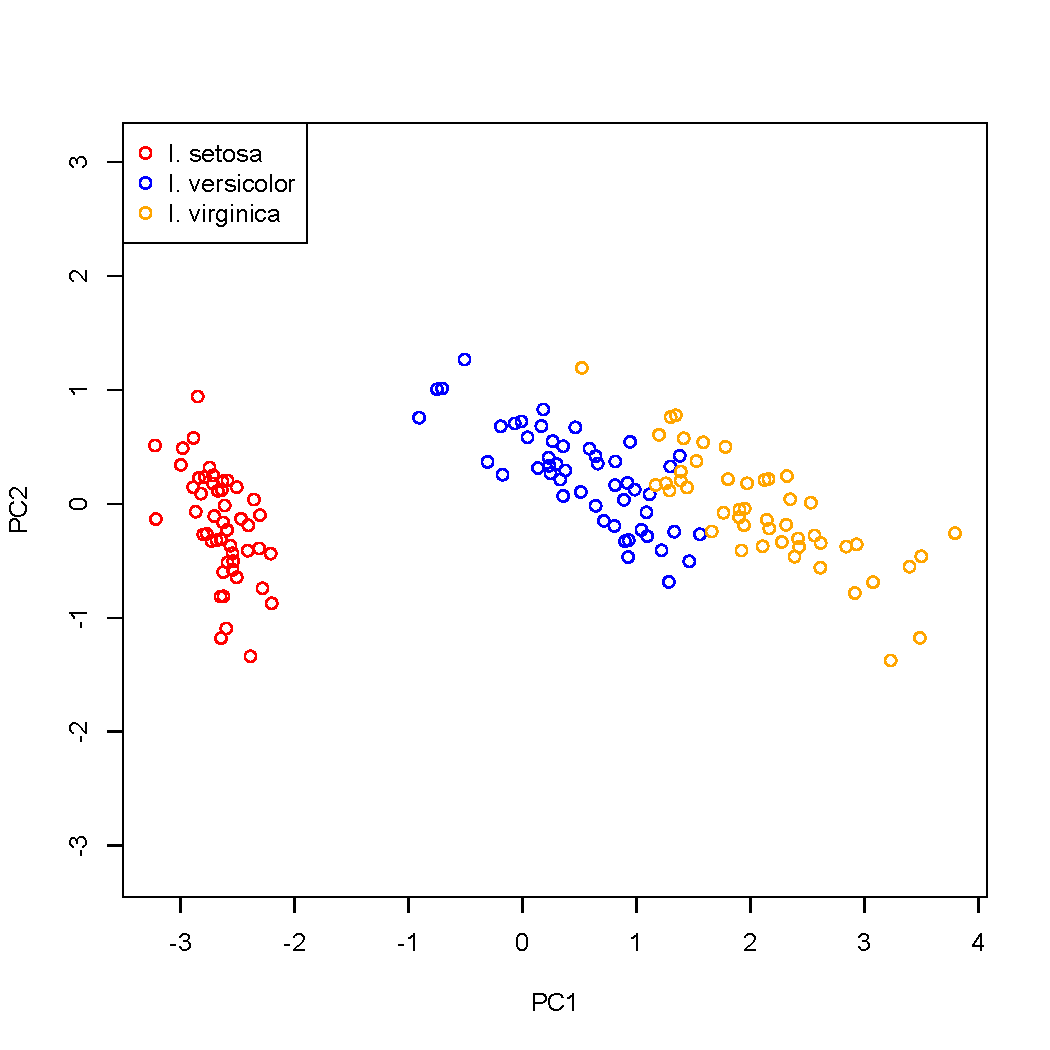
\includegraphics[width=0.8\columnwidth]{./figures/hands-on5/iris-all-pca.pdf}
\caption{PCA of the iris data set. One of your assignments is to
reconstruct this figure on your own.}
\end{figure}

